\documentclass[journal]{IEEEtran}
\ifCLASSINFOpdf
\usepackage[pdftex]{graphicx}
\else
\fi
\usepackage{amsmath}
\usepackage{amssymb}
\usepackage{amsthm}
\usepackage{bm}
\usepackage{mathrsfs}
\hyphenation{La-grange La-grang-ian dy-nam-ics}
\newcommand{\bma}[1]{\left[\begin{array}{#1}}
\newcommand{\ema}{\end{array}\right]}
\newcommand{\trans}{{\ensuremath{\mathsf{T}}}} % transpose
\newcommand{\utimes}{ {\raisebox{-0.6ex}{ \kern-1.0ex\raisebox{0.6ex}{ \small $\mathsf{v}$}}} } % 
\newcommand{\onehalf}{\mbox{$\textstyle{\frac{1}{2}}$}}
\DeclareMathAlphabet{\mbf}{OT1}{ptm}{b}{n}
\newcommand{\mbs}[1]{{\boldsymbol{#1}}}
\newcommand{\mbfbar}[1]{{\bar{\mbf{#1}}}}
\newcommand{\mbfhat}[1]{{\hat{\mbf{#1}}}}
\newcommand{\mbftilde}[1]{{\tilde{\mbf{#1}}}}
\newcommand{\mbsbar}[1]{{\bar{\boldsymbol{#1}}}}
\newcommand{\mbshat}[1]{{\hat{\boldsymbol{#1}}}}
\newcommand{\mbstilde}[1]{{\tilde{\boldsymbol{#1}}}}
\newcommand{\pspace}{\mathbb{P}} 
\newcommand{\ura}[1]{{\underrightarrow{{#1}}}}
\newcommand{\vectrix}[1]{\ensuremath \underrightarrow{\boldsymbol{\mathcal{F}}}_{#1}}
\def\fdota{{\raisebox{-2pt}{\LARGE $\cdot$}}}
\def\fdotb{{\raisebox{-0.6ex}{ \kern0.2ex\raisebox{0.8ex}{\tiny $\hspace*{-1ex}\circ$}}}}
\def\fddota{{\raisebox{-2pt}{\LARGE $\cdot\hspace*{-0.2ex}\cdot$}}}
\def\fddotb{{\raisebox{-0.6ex}{ \kern0.2ex\raisebox{0.8ex}{\tiny $\hspace*{-1ex}\circ\circ$}}}}
\newcommand{\fdot}[1]{{^{\fdota{\mbox{\footnotesize${#1}$}}}}}
\newcommand{\fddot}[1]{{^{\fddota{\mbox{\footnotesize${#1}$}}}}}
\newcommand{\beq}{\begin{equation}}
\newcommand{\eeq}{\end{equation}}
\newcommand{\bdis}{\begin{displaymath}}
\newcommand{\edis}{\end{displaymath}}
\newcommand{\beqarray}{\begin{eqnarray}}
\newcommand{\eeqarray}{\end{eqnarray}}
\newcommand{\beqarraynn}{\begin{eqnarray*}}
\newcommand{\eeqarraynn}{\end{eqnarray*}}

\begin{document}

\title{Quad-Rotor Helicopter Kinematics and Dynamics Proposal}

\author{{Gregory Miller 50760004}}

\markboth{AER 540 -- Intermediate Dynamics, Fall 2014}
{}

\maketitle

\begin{abstract}
This document proposes the idea of analyzing the kinematics and dynamics of a quad-rotor helicopter
as it travels through a pre-determined flight path. This analysis serves as the course project for 
AER 540, Intermediate Dynamics, Fall 2014. 
\end{abstract}

\IEEEpeerreviewmaketitle

\section{Introduction and Motivation}
\label{sec:intro_section}

\IEEEPARstart{A}{}quad-rotor helicopter is a flying device that has four horizontal spinning
rotors which produce the upward thrust needed to life the center piece, or body of the 
helicopter, into the air. See Figure \ref{fig:quad_intro} below, courtesy of website \cite{quad_intro},
for a visual example of a quad-rotor helicopter:

\begin{figure}[ht]
    \centering
        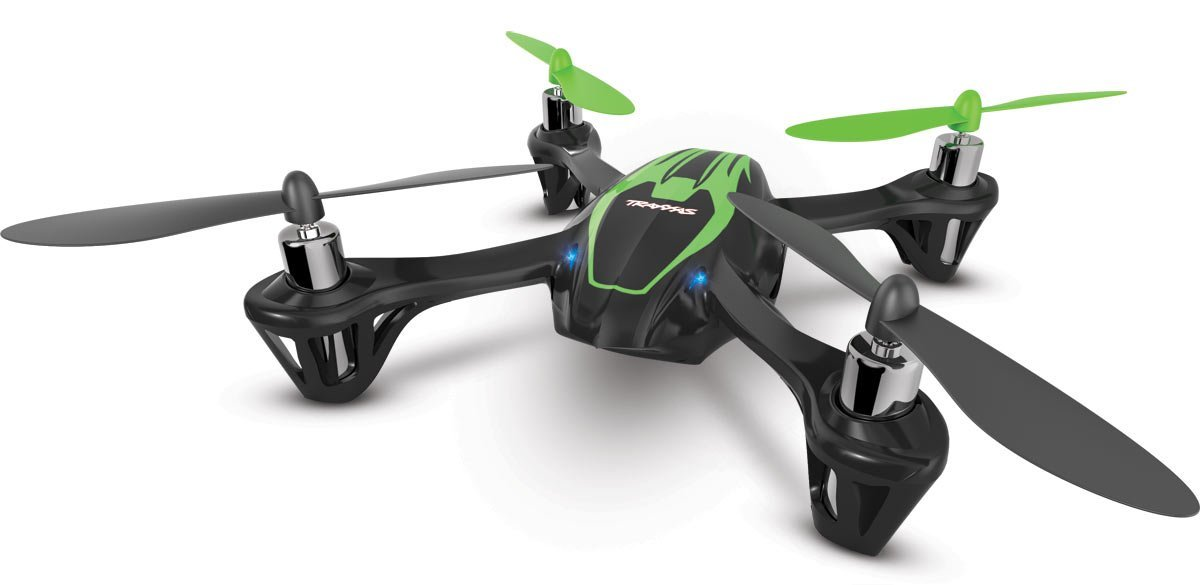
\includegraphics[width=.25\textwidth]{quad_intro}
    \caption{A visual example of a quad-rotor helicopter. Notice the four rotors.}
    \label{fig:quad_intro}
\end{figure}

The purpose of this course project is to analyze the kinematics and dynamics of a quad-rotor
helicopter as it flies through a pre-determined flight path. The inspiration for this
project came from the Michigan Autonomous Aerial Vehicles Club (MAAV). Every year,
the club designs and constructs a quad-rotor helicopter to compete in a competition
the subsequent August. In this competition, the goal is to have the quad-rotor
helicopter autonomously navigate its own way through an obstacle course. As no
human navigation input into the helicopter is allowed, its processor must use controllers
that can successfully command the helicopter's actuators, i.e., the four spinning
rotors, to direct the helicopter through its path. As such, it would be useful to 
model the quad-rotor helicopter's kinematics and dynamics as this information is
needed in order to design the controllers to produce steady and stable flight through the
obstacle course.   

\section{Kinematics of the Quad-Rotor Helicopter}
\label{sec:kinematics_section}

Kinematics refers to the geometry of motion of a moving object. For the quad-rotor
helicopter, it will follow a line for its pre-determined flight path. The characteristics
of the flight path line may include:

\begin{enumerate}
\item Straight segments.
\item Curved segments.
\item Vertical/Horizontal motion.
\item Upward/Downward motion that is angled with respect to the ground.
\end{enumerate}

The exact positions of the aggregate points that define the flight path line need to be
known in order to analyze the velocities and accelerations of the helicopter. This 
position information is important because, for example, the helicopter would experience,
for a fixed speed, significantly larger accelerations if its flight path 
curved excessively as opposed to smaller accelerations over only a slightly curved path. 

Consideration also needs to be given to the frame of reference fixed to the
helicopter body. This frame of reference may tilt or rotate with respect to the ground
frame as needed to have the helicopter maneuver itself through the obstacle course. 

\section{Dynamics of the Quad-Rotor Helicopter}
\label{sec:dynamics_section}

Dynamics refers to the forces that act upon an object and the resulting motion. 
A few considerations need to be taken into account for this portion of the analysis:

\begin{enumerate}
\item The weight of the quad-rotor helicopter. 
\item The four spinning rotors which produce four upward thrust forces that do not point
through the center of mass of the helicopter body. Thus opportunities for moments
arise.
\item The thrust magnitudes of the four rotors determine whether the helicopter moves
upward, downward, remains stationary with respect to the vertical direction, or tilts. 
\item The helicopter needs to tilt to have the four spinning rotors produce the
horizontal force components needed to maneuver the helicopter forward.
\item Any helicopter rotation will compromise any control as the helicopter's motion
depends on the relative positions of its rotors.
\item The drag that is imposed on the helicopter by the surrounding air.  
\end{enumerate}

During the dynamics analysis phase of the project, more considerations may need to be
taken into account. 

\section{Conclusion}
In this proposal, an introduction to quad-rotor helicopters was given along with 
the motivation for analyzing its kinematics and dynamics. After, details of what
the kinematics and dynamics analysis could entail were provided. 

\bibliographystyle{IEEEtran}
\bibliography{540_refs}

\end{document}


